\subsection{pitch shifting}
        \begin{frame}{pitch shifting}{standard approach}
            \begin{itemize}
                \item   \textbf{definition}:\\ change pitch without changing tempo
                \pause
                \item   \textbf{method}:\\ combine stretching and \textit{sample rate conversion} (interpolation)
                    \begin{enumerate}
                        \item   change length with stretching
                        \item   resample to compensate for length difference
                    \end{enumerate}
                \item<2->	\textbf{implementation}: differentiate ``external'' and ``internal'' parameters 
                        \begin{itemize}
                            \item	\textit{extern}: stretch $s_e$ and pitch $p_e$
                            \item	\textit{intern}: stretch $s_i$ and resample $r_i$
                        \end{itemize}
                
                \item<3-> \textbf{example}: pitch shift factor \textbf{$p = \nicefrac{4}{3}$}
					\begin{enumerate}
						\item	\textit{time stretch} (increase length/decrease tempo) $s = \nicefrac{4}{3}$
						\pause
						\item	\textit{resample} (decrease length, increase pitch) $r = \nicefrac{3}{4}$
                        \pause
                        \item[$\Rightarrow$]   audio:
                            \begin{itemize}
                                \item   OLA \includeaudio{audio/cathyOLApitch.mp3}
                                \item   phase vocoder \includeaudio{audio/cathypvpitch.mp3}
                            \end{itemize}
					\end{enumerate}
            \end{itemize}
        \end{frame}
        \begin{frame}{pitch shifting}{standard approach: stretch, pitch, resample factor examples}
			\setbeamercovered{invisible}

                \begin{itemize}
					\item	extern: $s_e=1$ $p_e=2$
					\pause
					\item[]	intern: $s_i=2$ $r_i=\frac{1}{2}$
					\pause
					\item	extern: $s_e=1$ $p_e=\frac{4}{3}$
					\pause
					\item[]	intern: $s_i=\frac{4}{3}$ $r_i=\frac{3}{4}$
					\pause
					\item	extern: $s_e=\frac{1}{2}$ $p_e=2$
					\pause
					\item[]	intern: $s_i=1$ $r_i=\frac{1}{2}$
					\pause
					\item	extern: $s_e=2$ $p_e=2$
					\pause
					\item[]	intern: $s_i=4$ $r_i=\frac{1}{2}$
				\end{itemize}
  			\setbeamercovered{transparent}
      \end{frame}
        \begin{frame}{pitch shifting}{frequency domain approach}
            \begin{enumerate}
                \item   STFT
                \item<2->   magnitude and phase
                \item<3->   magnitude and instantaneous frequency
                \item<4->   resample both magnitude and frequency spectrum acc.\ to pitch factor
                \item<5->   magnitude and phase
                \item<6->   complex spectrum
                \item<7->   IFFT and OLA
            \end{enumerate}
        \end{frame}
        \subsection{formant preservation}   
        \begin{frame}{pitch shifting}{formant preservation: time domain}
	\begin{itemize}
		\item 	\textbf{idea}
			\begin{itemize}
				\item 	signal is pulse train filtered by transfer function
					\pause
					\begin{itemize}
						\item 	pulse train determines fundamental frequency
						\item	transfer function determines formant shape/timbre characteristics
					\end{itemize}
			\end{itemize}
		\pause
        \bigskip
		\item	\textbf{approach}
			\begin{itemize}
				\item	change grain/pulse distance
				\item	grain ``content'' not modified\\ $\rightarrow$ freq domain not modified
				\pause
                \bigskip
				\item[$\Rightarrow$]	\textbf{``same'' spectrum,\\ different pitch}
			\end{itemize}
	\end{itemize}
    \vspace{-30mm}
        \visible<3->{
                    \begin{flushright}
                        \hspace{10mm}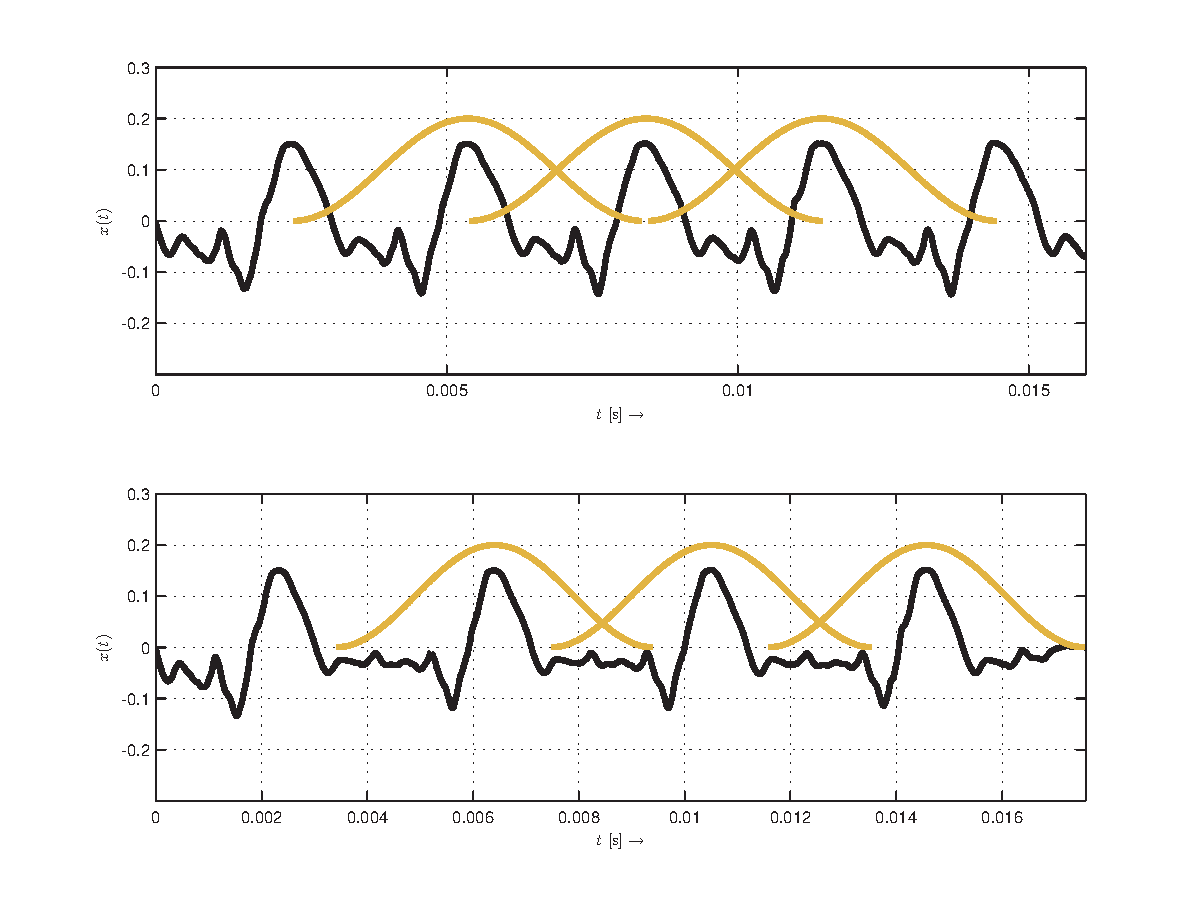
\includegraphics[scale=.25]{graph/PsolaPitch}
                    \end{flushright}   
                    }
        \end{frame}
        \begin{frame}{pitch shifting}{formant preservation: frequency domain}
           \begin{columns}
                \column{.5\textwidth}
                    \begin{itemize}
                        \item \textbf{idea}
                            \begin{itemize}
                                \item   preserve spectral envelope
                            \end{itemize}
                        \bigskip
                        \pause
                        \item \textbf{approach}
                            \begin{enumerate}
                                \item   measure spectral envelope
                                \item   apply inverse envelope (whitening)
                                \item   pitch shift
                                \item   apply spectral envelope
                            \end{enumerate}
                  \end{itemize}
                \column{.5\textwidth}
        \visible<3->{
                    \begin{figure}
                        \centering
                        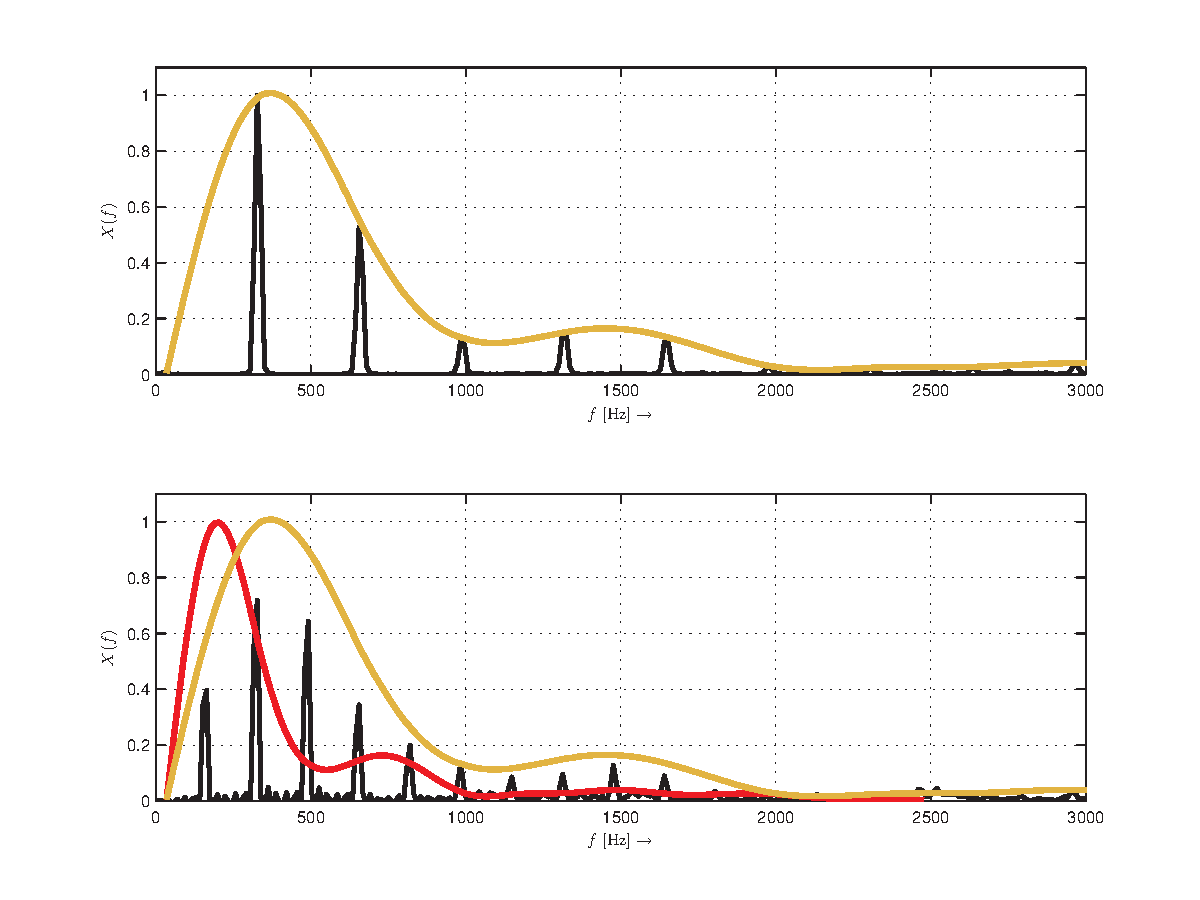
\includegraphics[scale=.25]{graph/SpectralEnvelope}
                    \end{figure}   
                }
            \end{columns}
        \end{frame}
        \begin{frame}{pitch shifting}{spectral envelope estimate}
            \begin{itemize}
                \item   \textbf{approaches}
                    \begin{itemize}
                        \item   LPC coefficients
                        \item   spectral maxima
                    \end{itemize}
                \pause
                \bigskip
                \item   \textbf{potential issues}
                    \begin{itemize}
                        \item   \textit{polyphonic input} audio:\\ 'superposition' of envelopes
                        \item   \textit{very high/low pitch factors}: high frequency boost/cut
                        \item   \textit{estimate resolution}
                            \begin{itemize}
                                \item   too coarse $\rightarrow$ loss of timbre characteristics
                                \item   too fine $\rightarrow$ impress pitch characteristics (harmonic pattern) on spectrum
                            \end{itemize}
                    \end{itemize}
            \end{itemize}
        \end{frame}
        \begin{frame}{pitch shifting}{audio examples}

                    \begin{columns}
                        \column{.33\textwidth}
                        \textbf{OLA}
                            \begin{itemize}
                                \item   orig \includeaudio{audio/cathy.mp3}
                                \item   resample $p = \nicefrac{4}{3}$\includeaudio{audio/cathyOLApitch.mp3}
                                \item   \color{gtgold}{formant} $p = \nicefrac{4}{3}$\includeaudio{audio/cathyOLApitchf.mp3}
                            \end{itemize}
                        \column{.33\textwidth}
                        \textbf{PSOLA}
                            \begin{itemize}
                                \item   orig \includeaudio{audio/cathy.mp3}
                                \item   resample $p = \nicefrac{4}{3}$\includeaudio{audio/cathySOLpitch.mp3}
                                \item   formant $p = \nicefrac{4}{3}$\includeaudio{audio/cathySOLpitchf.mp3}
                            \end{itemize}

                        \column{.33\textwidth}
                        \textbf{PVOC}
                            \begin{itemize}
                                \item   orig \includeaudio{audio/cathy.mp3}
                                \item   resample $p = \nicefrac{4}{3}$ \includeaudio{audio/cathyPropitch.mp3}
                                \item   formant $p = \nicefrac{4}{3}$ \includeaudio{audio/cathyPropitchf.mp3}
                            \end{itemize}
                    \end{columns}        
                \end{frame}
